% Preamble
% ---
\documentclass{article}

% Packages

\usepackage{graphicx}
\usepackage{subfig}
\usepackage{pgfplots}

% ---


\graphicspath{ {assets/} }
\begin{document}


\section{Face detection}


TOGO
Limitation of TPR. Difficult to define "true" values. The bouding region of a
face is discrete and we may choose not to detect side on faces. Example below
shows 2 possible "true" values for a detection. One give a IOU of under 0.7 but
the other gives over 0.9.

% -- Part 1 - Image section
\begin{figure}
\begin{tabular}{ccc}
\subfloat[dart4]{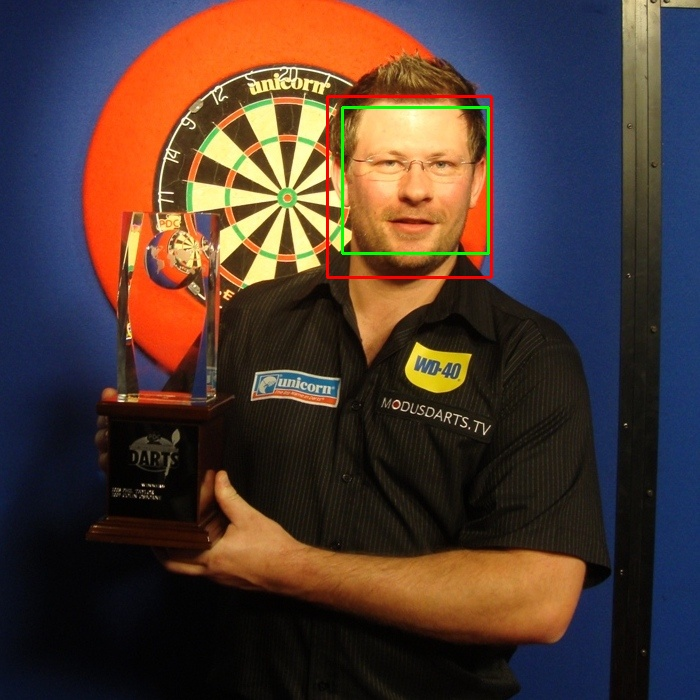
\includegraphics[width = 1.4in]{dart4-face}} &
\subfloat[dart5]{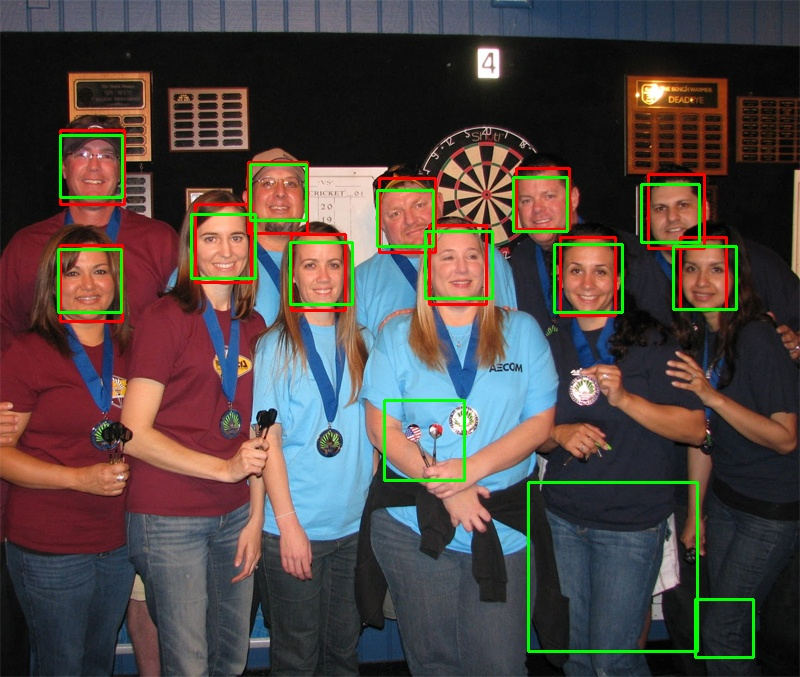
\includegraphics[width = 1.4in]{dart5-face}} &
\subfloat[dart13]{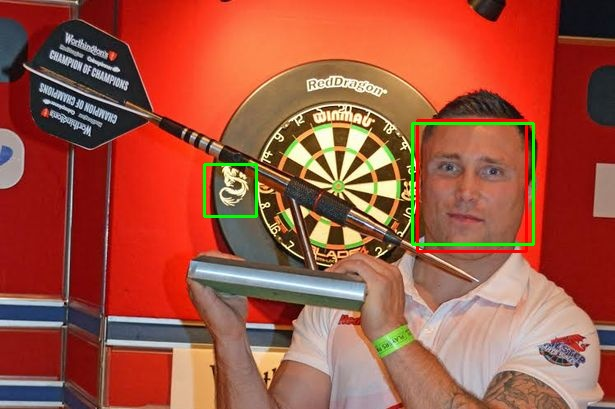
\includegraphics[width = 1.4in]{dart13-face}} \\
\subfloat[dart14]{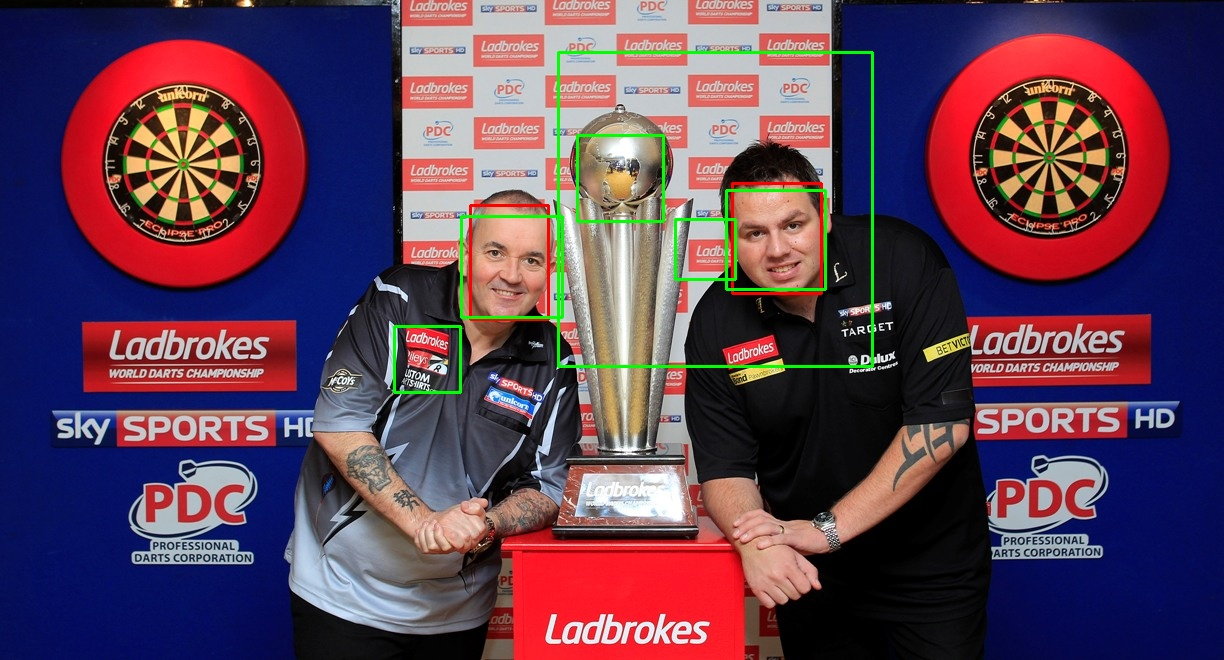
\includegraphics[width = 1.4in]{dart14-face}} &
\subfloat[dart15]{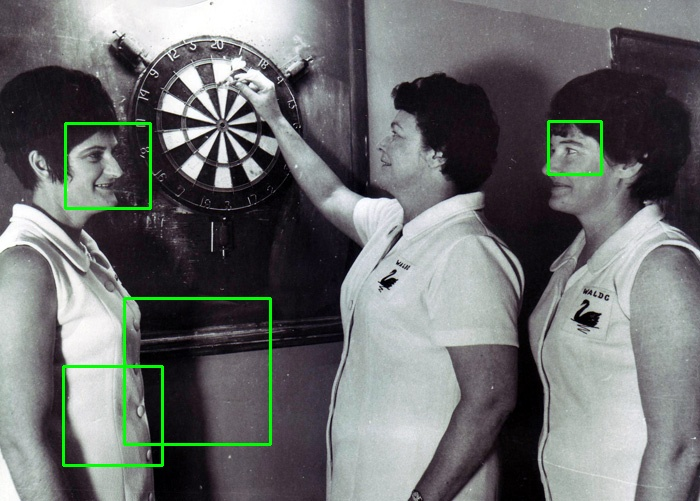
\includegraphics[width = 1.4in]{dart15-face}} &
\end{tabular}
\caption{Frontal face detection with ground truth}
\end{figure}

\bigskip

\begin{tabular}{ |p{3cm}||p{3cm}|p{3cm}| }
 \hline
 \multicolumn{3}{|c|}{Frontal face detection results} \\
 \hline
 Image name & TPR & F1-SCORE \\
 \hline
 dart4  & 1   & 1         \\
 dart5  & 1   & 0.88      \\
 dart13 & 1   & 0.666667  \\ 
 dart14 & 1   & 0.5       \\ 
 dart15 & 1   & 0         \\ 
 \hline
\end{tabular}

\bigskip

The results show that the true positivity rate, TPR, for all images is 1.
Despite this we often see far lower F1 scores. This reveals the limitation of
the TPR as a detector can always achieve a high TPR by having a low tolerance
to classify something as a face. This would result in a very low F1 score as
many false positives would arise yet the true positivity rate would remain
high.

The image dart-15 reveals another limitation of these metrics. It can often to
difficult to classify the ground truth. This classifier was created to detect
frontal faces and therefore in dart15 I have claimed no frontal face present.
Despite this the classifier has detected on of the faces brining its F1 score
down. Similarly there is no clear boundry for a face and therefore the exact
area that should be detected can vary resulting in the need for a larger
tolerance for the intersection over area, IOU.

\section{Dart board detection}

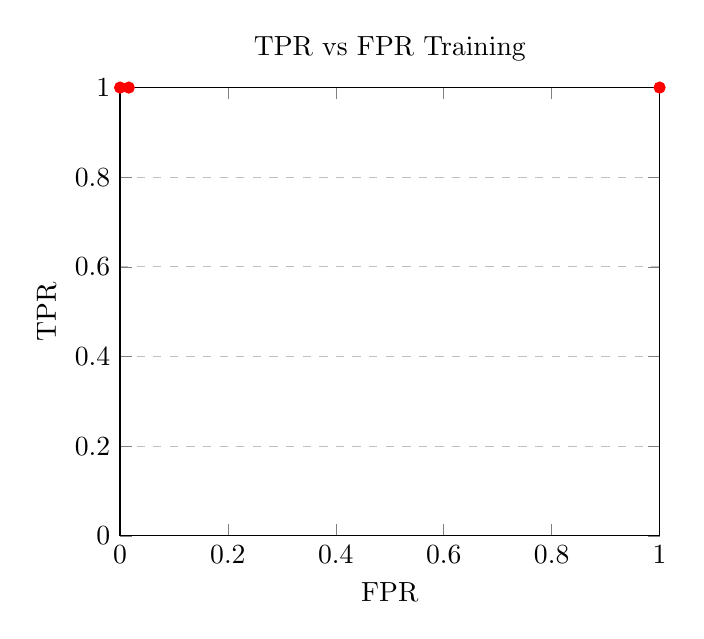
\begin{tikzpicture}
\label{tprvsfprtraining}
\begin{axis}[
    title={TPR vs FPR Training},
    xlabel={FPR},
    ylabel={TPR},
    xmin=0, xmax=1,
    ymin=0, ymax=1,
    xtick={0, 0.2, 0.4, 0.6, 0.8, 1.0 },
    ytick={0, 0.2, 0.4, 0.6, 0.8, 1.0 },
    legend pos=north west,
    ymajorgrids=true,
    grid style=dashed,
]

\addplot[
    color=red,
    only marks, 
    mark=*,
    ]
    coordinates {
      (1,1)(0.0163415,1)(0.000237497,1)
    };
    
\end{axis}
\label{fig:picture}
\end{tikzpicture}

Figure \ref{tprvsfprtraining} shows the change in FPR and TPR throughout the
training process. At the beginning of the training all images are accepted
throughout the stages more layers are added to the cascade. Each layer will
remove of the regions classified as a dart board. This results in a drop in FPR
as the training takes place. Throughout the training process the TPR remains
and 1. However if more layers were added (and therefore the classifier removed
more classified regions) then the TPR could also be reduced. This could still
result in the classifiers F1 score increasing as the FPR would also be
decreasing.

\begin{figure}
\label{dartdetectionimages}
\begin{tabular}{ccc}
\subfloat[dart1]{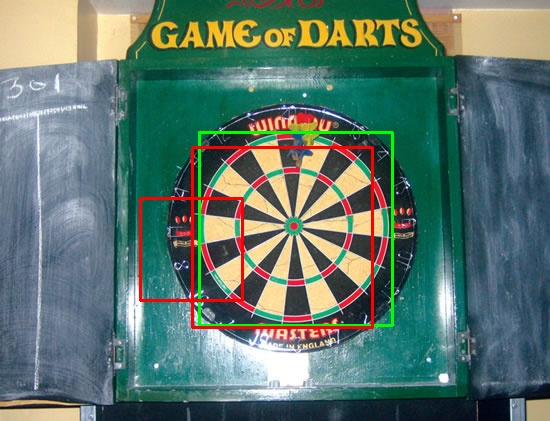
\includegraphics[width = 1.4in]{dart1-dart}} &
\subfloat[dart6]{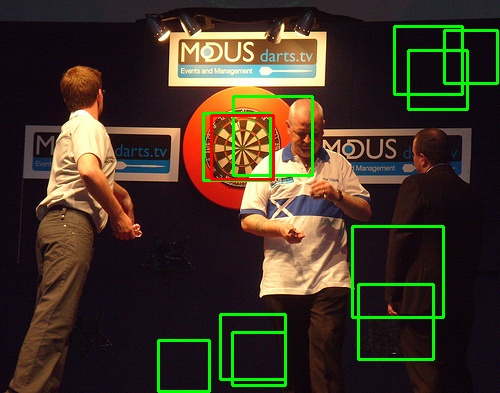
\includegraphics[width = 1.4in]{dart6-dart}} &  
\subfloat[dart4]{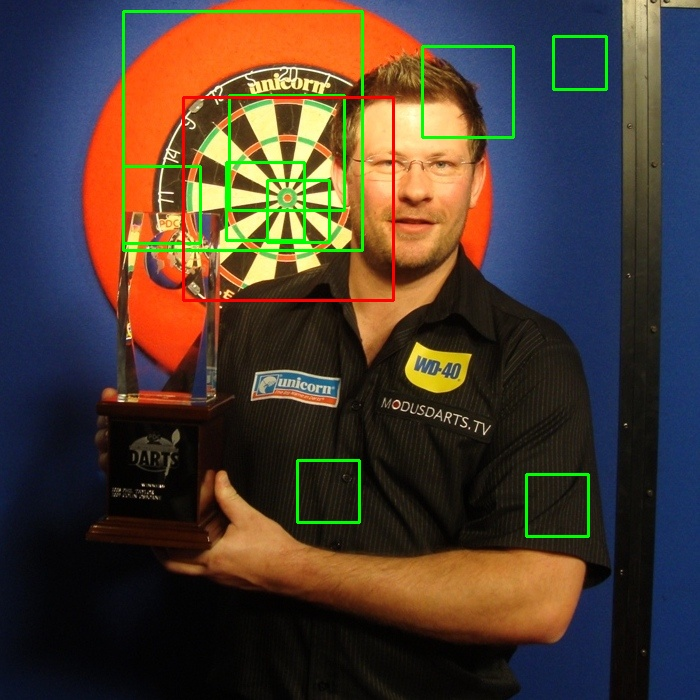
\includegraphics[width = 1.4in]{dart4-dart}} \\
\end{tabular}
\caption{Dart board detection with ground truth}
\end{figure}


\begin{tabular}{ |p{2cm}||p{2cm}|p{2cm}| }
\label{dartresults}
 \hline
 \multicolumn{3}{|c|}{Frontal face detection results} \\
 \hline
 Image name & TPR & F1-SCORE \\
 \hline
 dart1  & 1  & 0.666667   \\
 dart2  & 1  & 0.25       \\
 dart3  & 1  & 0.4        \\
 dart4  & 0  & 0          \\
 dart5  & 0  & 0          \\
 dart6  & 1  & 0.181818   \\
 dart7  & 0  & 0          \\
 dart8  & 0  & 0          \\
 dart9  & 0  & 0          \\
 dart10 & 0  & 0          \\
 dart11 & 0  & 0          \\
 dart12 & 0  & 0          \\
 dart13 & 0  & 0          \\
 dart14 & 0  & 0          \\
 dart15 & 1  & 0.5        \\
 \hline
 Average& 0.333333  & 0.133232    \\ 
 \hline
\end{tabular}

The average values in Table \ref{dartresults}, show the unreliable results of
the cascade for detecting dart boards.  It not only has a very low TPR and also
a very low F1-score suggesting there are many missed dart boards as well as
regions falsely classified. The images in Figure \ref{dartdetectionimages} show
the wide range of results from the classifier. a and b show successful
classifications yet b and c show the high number of false positives. It is also
noteworthy that the TPR values achieved during training were far higher than
the average achieved during testing. This is as a result of the method used to
generate positive images. These took one image of a dart board and generated
variations (via movements/rotations) on that image. This means when classifying
different types of dartboards of those with objects in the way (such as
\ref{dartresults} c) the classifier performs far worse.

\end{document}
